%% PNAStwoS.tex
%% Sample file to use for PNAS articles prepared in LaTeX
%% For two column PNAS articles
%% Version: Apr 15, 2008 
 

%% BASIC CLASS FILE
\documentclass{pnastwo}

%% ADDITIONAL OPTIONAL STYLE FILES
\usepackage{graphicx}
\usepackage{pnastwoF}
\usepackage{amssymb,amsfonts,amsmath}
\usepackage{subfig}
\usepackage{bm}
%\usepackage[comma,sort&compress]{natbib}
\usepackage{cite}
\renewcommand\citeleft{(} \renewcommand\citeright{)}

%% OPTIONAL MACRO DEFINITIONS
\def\s{\sigma}
\newcommand{\erf}{\operatorname{erf}}


%%%%%%%%%%%%
%% For PNAS Only:
\url{www.pnas.org/cgi/doi/10.1073/pnas.0709640104}
\copyrightyear{2008}
\issuedate{Issue Date}
\volume{Volume}
\issuenumber{Issue Number}
%\setcounter{page}{2687} %Set page number here if desired
%%%%%%%%%%%%

\begin{document}

\title{A model-based method for transcription factor target
  identification with limited data}

\author{Antti Honkela\affil{1}{Department of Information and Computer
    Science, Helsinki University of Technology, Finland}, Neil D.
  Lawrence\affil{2}{School of Computer Science, University of
    Manchester, UK}, Charles Girardot\affil{3}{Genome Biology unit,
    European Molecular Biology Laboratory, Heidelberg, Germany},
  Hilary Gustafson\affil{3}{}, Ya-Hsin Liu\affil{3}{}, Eileen
  E. Furlong\affil{3}{} \and Magnus Rattray\affil{2}{}}

\contributor{Submitted to Proceedings of the National Academy of Sciences
of the United States of America}

\maketitle

\begin{article}
\begin{abstract}
  We present a computational method for identifying potential targets of a
  transcription factor using wild-type gene expression time series
  data. For each putative target gene we fit a simple differential equation model
  of transcriptional regulation and the model likelihood serves as a
  score to rank targets. The expression profile of the transcription
  factor is modeled as a sample from a Gaussian process prior
  distribution that is integrated out using a non-parametric
  Bayesian procedure. This results in a parsimonious model with relatively few
  parameters which can be applied to short time series data
  sets without excessive over-fitting. We assess our method using
  genome-wide Chromatin Immunoprecipitation
  (ChIP-chip) and loss-of-function mutant expression data for two
  transcription factors controlling early mesoderm development in Drosophila. Lists of top-ranked
  genes identified by our method are significantly enriched for genes
  close to bound regions identified in the ChIP-chip data and significantly
  enriched for genes that are differentially expressed in
  loss-of-function mutants. Our approach is found to be superior to
  ranking using mutant differential expression scores and mostly
  superior to an approach based on correlation with transcription factor
  expression. We also show how integrating complementary wild-type
  spatial expression data can further improve target ranking performance.
\end{abstract}

\keywords{transcriptional regulation | gene expression | systems biology | Gaussian process inference}

\abbreviations{TF transcription factor; ChIP Chromatin Immunoprecipitation;}

\dropcap{T}ranscription factors are key nodes in the gene regulatory
networks that determine the function and fate of
cells. An important first step in uncovering a gene regulatory network
is the identification of target genes regulated by a specific
transcription factor (TF). A
common approach to this problem is to experimentally locate physical binding
of TF proteins to DNA sequence {\em in vivo} using a genome-wide
chromatin immunoprecipitation (ChIP) experiment~\cite{Ren2000,Iyer2001}. However, recent studies have shown that many observed binding events are neutral and do not regulate transcription, while regulatory binding events often occur at enhancers that are not proximal to the target gene that they control~\cite{Li2008,MacArthur2009}. Therefore, the task of identifying transcriptional
targets requires the integration of ChIP binding predictions
with evidence from expression data to help associate binding events
with target gene regulation. If there is access to expression data from a mutant in which the TF has
been knocked out or over-expressed, then differential expression of genes between wild-type
and mutant is indicative of a potential regulatory
interaction~\cite{Furlong2001}. Available spatial expression data for the
TF and putative target can also provide support for a hypothesised
regulatory link. 

A problem with the above approach is that the creation of mutant
strains is challenging or impossible for many TFs of interest. Even
when viable mutants are available then they may provide very limited information because of redundancy or due to the
confounding of signal from indirect regulatory feedback~\cite{Gitter2009}. For these reasons it
is useful to seek other sources of evidence to complement ChIP binding
predictions. In this contribution we demonstrate how a dynamical model of wild-type transcriptional
regulation can be used for genome-wide scoring of putative target genes. All that is required to apply
our method is wild-type time series data collected over a period
where TF activity is changing. Our approach allows for complementary
evidence from expression data to be integrated with ChIP binding data
for a specific TF without carrying out TF perturbations. 

To score putative targets we use the data likelihood under a simple
cascaded differential equation model of transcriptional regulation. The regulation model
we apply is ``open'' in the sense that we do not explicitly model regulation of the TF
itself. To deal with this technical issue we use a recently developed
non-parametric probabilistic inference methodology to
effectively deal with open differential equation
systems~\cite{Gao2008}. We model the TF concentration as a function
drawn from a Gaussian process prior distribution~\cite{Rasmussen2006}. This functional prior can either be placed
on the TF mRNA, for TFs primarily under transcriptional regulation,
or the TF protein, for TFs activated post-translationally. In the
application considered here the TFs are transcriptionally regulated
and we take the former approach. We use Bayesian marginalisation (also
known as Bayesian model averaging) to
integrate out this functional degree of freedom. This greatly reduces the
number of parameters required to model the data, making a
likelihood-based approach feasible even for short time series
datasets. 

There are many existing approaches to inferring gene regulatory networks from
time series expression data, including dynamic Bayesian networks,
information theoretic approaches and differential equation approaches
(reviewed in \cite{Bansal2007a}). These methods typically require many
more data from a greater diversity of experimental conditions than are
available from the short unperturbed wild-type time series that we
consider. Indeed, most real gene expression time course data are short
relative to the simulated data used to assess computational methods
for network inference~\cite{Ernst2005}. However, our goal is more limited in scope since
we are primarily interested in providing additional support for hypothesised
targets of a specific TF. Again, most approaches to this problem are
designed for data containing large numbers of diverse conditions, as
exemplified by the DREAM 2 target identification
challenge 1~\cite{Stolovitzky2007}. Others
have addressed this target identification problem using time series
data with a regulation model~\cite{Barenco2006a,Gatta2008}. However,
these approaches either require a known target set for training~\cite{Barenco2006a} or
they require measured TF protein data~\cite{Gatta2008}. As well as
these differences in the assumed prior knowledge and data available,
it is also difficult to validate other approaches on the same data used in these
studies as they only carried out validation of positive targets
that they identified, rather than using unbiased genome-wide
experimental validation. 

We validate our proposed method by comparing the model-based target
ranking with published ChIP-chip data for two TFs controlling early
mesoderm development in Drosophila. Our method is shown to be comparable
to, or outperform, the use of knockout mutant data which are available
for these TFs. We demonstrate that a model-based approach is significantly
better than a simpler approach using correlation with TF
expression. We further show how integrating complementary wild-type spatial
{\em in situ} expression data can greatly improve target ranking accuracy. 

\begin{figure*}[tb]
  \centering
  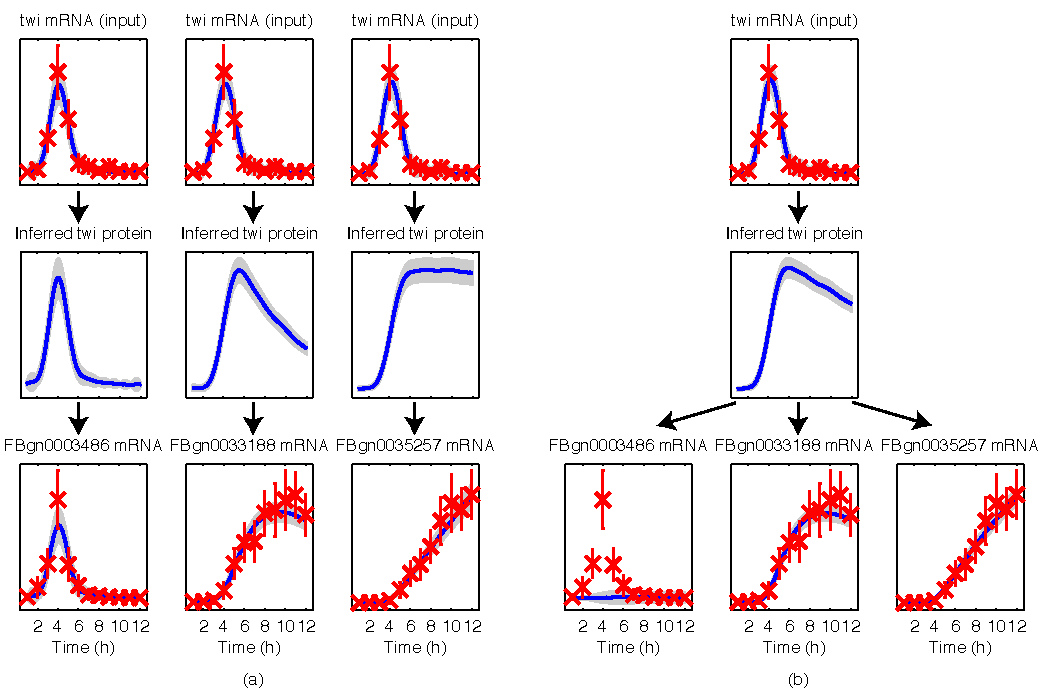
\includegraphics{dros_gpdisim_models}
  \caption{(a) Three independent single-target Gaussian process models
    for likely targets of the TF Twist. Red marks denote observed expression
    levels with 2 s.d.\ error bars while blue functions are inferred
    from the model.  The shaded regions denote 2 s.d.\ confidence
    intervals. (b) A joint multiple-target Gaussian process model for
    the same set of target genes as in (a). It should be noted that
    the multiple-target models used in evaluation have more targets
    than the one shown here.\label{fig:gpdisim_models}
}
  %\label{fig:gpdisim_models}
\end{figure*}

\section{Gaussian process inference for a linear activation model}

A Gaussian process is a probability distribution over
functions $f$ which take the value $f(t)$ at time
$t$. Analogous to the Gaussian distribution, which is fully
characterised by a mean and covariance, the Gaussian process is
characterised by a mean function $\mathrm{E}[f(t)]$ and a covariance
function $k(t,t')=\mathrm{E}[f(t)f(t')]-\mathrm{E}[f(t)]\mathrm{E}[f(t')]$
where the expectation is over function evaluations at times $t$ and
$t'$. 

For the prior distribution of TF mRNA concentration profile $f$ we use a zero-mean squared exponential covariance
$k(t,t')=a\exp(-(t-t')^2/l^2)$. Samples from a Gaussian process with this choice
of covariance are smooth, infinitely differentiable, stationary functions. Although single-cell mRNA counts may be low
and vary in a highly stochastic manner, here we consider microarray data which
corresponds to a population average and is therefore more
appropriately modeled using a smooth process. The parameters $a$ and
$l$ describe the typical amplitude and time-scale of samples from
the prior. 

To simplify the inference we model translation and transcriptional
activation as simple linear processes using ordinary differential
equations,
\begin{align}
  \frac{\mathrm{d}p(t)}{\mathrm{d}t} & = f(t) - \delta
  p(t) \ , \label{eq:translation_ode} \\
  \frac{\mathrm{d}m_j(t)}{\mathrm{d}t} & = B_j+S_j p(t)-D_j m_j(t) \ , \label{eq:transcription_ode}
\end{align}
where $p(t)$ is the TF protein and $m_j(t)$ is the $j$th target mRNA
concentration at time $t$. The parameters $B_j$, $S_j$ and $D_j$ are the
baseline transcription rate, sensitivity and decay rate respectively
for the mRNA of the $j$th target (as described in \cite{Barenco2006a}).
The parameter $\delta$ is the decay rate of the TF protein.
This linear system of differential equations can be
explicitly solved and we find that the functions $p$ and $m_j$ are
linear functions of $f$. Given $k$ target genes the functions $f$ and $\bm m\equiv[m_j]$ therefore
describe a $k$+1-dimensional Gaussian process prior $p(f,\bm m|\theta)$
for which the covariance function can be calculated explicitly in terms of the
$3$ global and $3k$ gene-dependent model parameters
$\theta=[\delta,a,l,\{B_j,S_j,D_j\}]$ (see Materials and Methods). 

A microarray time course experiment provides a data vector $\bm y$ containing the noise-corrupted TF and target mRNA
measurements at $n$ times,
$\bm
y=[\hat{f}(t_1),\hat{f}(t_2),\ldots,\hat{f}(t_n),\{\hat{m}_j(t_1),\ldots,\hat{m}_j(t_n)\}]^\mathrm{T}$. This
is a continuous-time modeling framework so there is no
requirement that times are equally spaced. We assume Gaussian noise:
$p(\bm y|f,\bm m)=\prod_i{\cal
  N}(\hat{f}(t_i)|f(t_i),\sigma_{if}^2)\prod_j{\cal
  N}(\hat{m_j}(t_i)|m_j(t_i),\sigma_{ijm}^2)$ where the gene and condition
specific measurement variance parameters $\sigma_{if}^2$ and
$\sigma_{ijm}^2$ are obtained from a probe-level analysis of the
microarray data~\cite{Liu2005,Pearson2009} (see
Materials and Methods). The log-likelihood for the model parameters
$\theta$ can then be calculated exactly using standard Gaussian process regression
techniques to integrate out the functions $\bm m$ and
$f$~\cite{Rasmussen2006}. For $R$ replicate datasets the
log-likelihood is
\begin{equation*}
  \begin{split}
    L(\theta) & = \log p(\bm y_1,\bm y_2,\ldots,\bm y_{R}|\theta) \\
    & = \sum_{r=1}^{R} \log \!\int 
    \!\!p(\bm y_r|f,\bm m)p(f,\bm m|\theta) \, \mathrm{d}\!f\mathrm{d}\bm m\\
    & = \sum_{r=1}^{R} \left[-\frac{1}{2}\bm y_r^\mathrm{T} K_r^{-1} \bm y_r -
      \frac{1}{2}\log|K_r|\right] -nR\log 2\pi
  \end{split}
\end{equation*}
where $K_r$ is the covariance matrix for the
noise-corrupted dataset $\bm y_r$ under the Gaussian process prior (see
Materials and Methods). This allows us to compute the set of model
parameters $\theta$ by maximum
likelihood using gradient-based optimisation. 

Rather than assuming that the TF protein is primarily under
transcriptional control, as indicated by
Eq.~(\ref{eq:translation_ode}), one can alternatively use the idea pioneered
in~\cite{Barenco2006a} and model the TF protein as an unobserved
latent variable. This approach can naturally be carried out using a
similar Gaussian process framework as shown in~\cite{Gao2008}. However, that procedure requires a set of known
targets for training the model whereas the approach described above
can be applied without any prior knowledge of targets. We therefore
prefer the above cascade model for cases where the level of active TF is under direct transcriptional control. 

\section{Results}

We applied our model-based approach to identify targets of the TFs
Twist and Mef2 which regulate mesoderm and muscle development in
Drosophila~\cite{Sandmann2007,Zinzen2009}. We used a microarray dataset
containing three replicated time series of 12 time points collected
hourly throughout Drosophila embryogenesis using wild-type
embryos~\cite{Tomancak2002}.  Quiet candidate targets were eliminated by 
considering average z-scores of expression values as described in
Materials and Methods.

For each TF we fitted two sets of Gaussian process models. In one
approach all other genes were considered as individual candidate targets one at a
time (``single-target models'').  The candidate targets were ranked
according to their likelihood under the model.  It is worth noting that even the global
parameters can vary between models for different genes under this approach as the models
are fitted completely independently. In an alternative approach we fitted another set of models using the five
top-ranking genes in the single-target case as the training set (``multiple-target models''; see
Materials and Methods).  An illustration comparing these alternative
modeling approaches is shown in Fig.~\ref{fig:gpdisim_models}. The
single-target model is more flexible because each
potential target gene can be associated with a different inferred TF
protein profile. The multiple-target model is constrained to explain
all targets with the same TF protein profile and may therefore assign
a low score to targets that have a high score according to the
single-target model (this is the case for gene FBgn0003486 in
Fig.~\ref{fig:gpdisim_models}). Nevertheless, both models are
sufficiently flexible to fit target genes with significantly different
profiles (genes FBgn0033188 and FBgn0035257 in
Fig.~\ref{fig:gpdisim_models}).

For comparison, candidates were also ranked by correlation of the
expression profile with the TF expression profile (``correlation'')
and by $q$-value of differential expression in TF loss-of-function mutant
experiments from~\cite{Sandmann2006a,Sandmann2007} (``knock-out''). 

\begin{figure}[tb]
  \centering
  %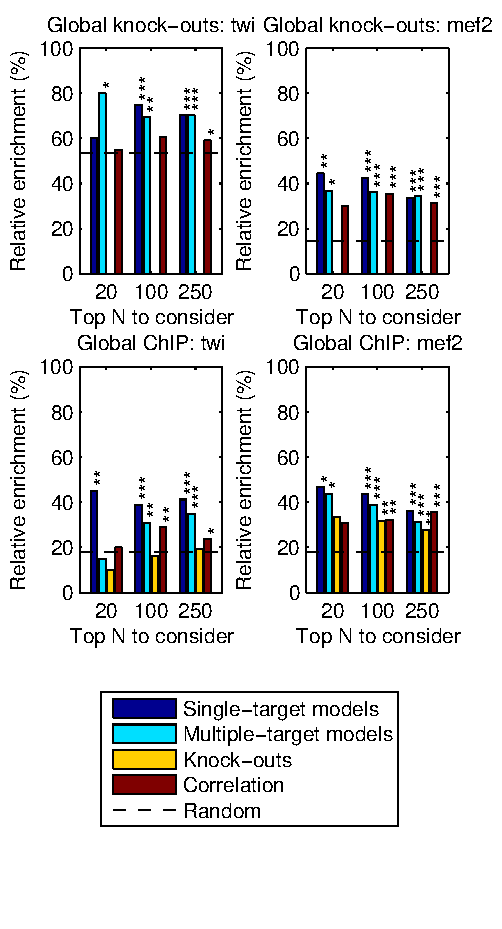
\includegraphics[trim=0mm 18mm 0mm 0mm]{dros_global_evaluation}
  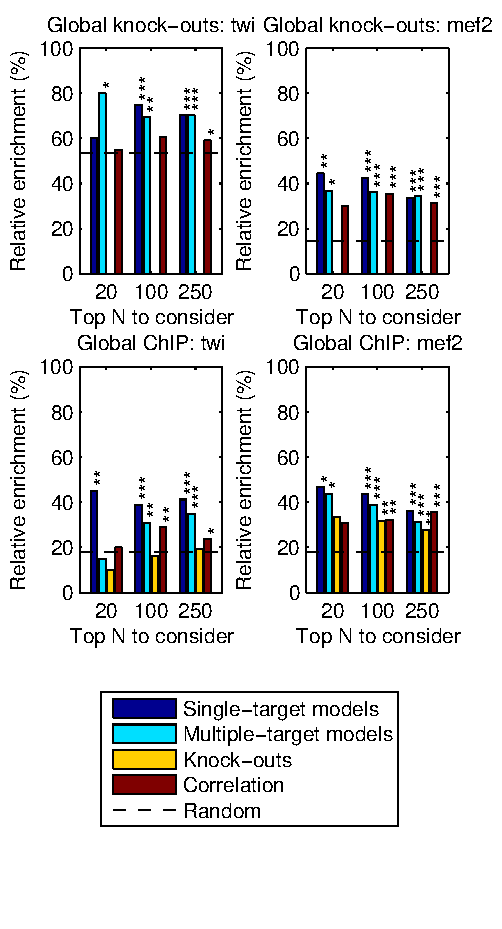
\includegraphics{dros_global_evaluation}
  \caption{Global evaluation results of different rankings as
    discussed in the text showing the relative frequency of positive
    predictions among $N$ top-ranking targets.
    The dashed line
    denotes the frequency in the full population.
    The first row shows the frequency of targets with ChIP-chip
    binding within 5000 base pairs of the gene
    while the second row shows the frequency of
    predicted targets with significant differential
    expression in TF knock-outs.
    $p$-values of results significantly different from random are
    denoted by `***': $p <
    0.001$, `**': $p < 0.01$, `*': $p < 0.05$.
    Comparison to knock-out ranking is obviously omitted for knock-out
    validation. \label{fig:dros_global_evaluation}
  }
 % \label{fig:dros_global_evaluation}
\end{figure}

The accuracy of the ranking was evaluated by looking at the global
fraction of $N$ top-ranking targets that are significantly
differentially expressed in knock-outs of the TFs and the fraction
of targets with ChIP-chip binding within 5000 base
pairs of its beginning or end or within the gene in the data
from~\cite{Zinzen2009}. Both of our model-based approaches are found to
be superior to the knock-out results in terms of ChIP binding
enrichment and are mostly superior to the correlation results in terms
of both ChIP binding enrichment and knock-out differential expression
(see Fig.~\ref{fig:dros_global_evaluation}). The model-based ranking
results also show a consistently high level of significance. The
single-target models perform slightly better than the multiple-target
models in most cases.

\begin{figure}[tb]
  \centering
  %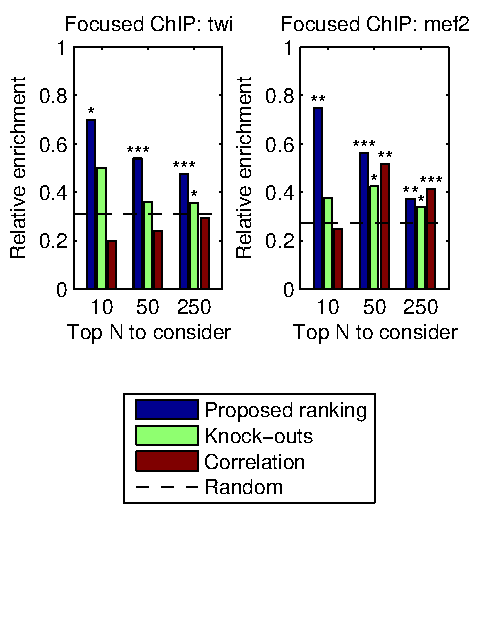
\includegraphics[trim=0mm 8mm 0mm 0mm]{dros_focused_evaluation}
  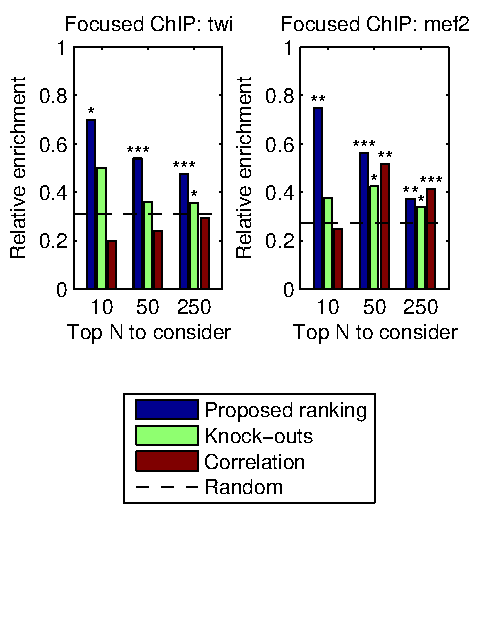
\includegraphics{dros_focused_evaluation}
  \caption{Evaluation results of different rankings based on
    ChIP-chip data similar to those in
    Fig.~\ref{fig:dros_global_evaluation} except only for genes
    with annotate expression in mesoderm and muscle.
%     as discussed in the text showing the relative frequency of
%     positive predictions among $N$ top-ranking targets.  The dashed
%     line denotes the frequency in full population.  The first row
%     shows the frequency of predicted targets that are significantly
%     differentially expressed in knock-outs for the TF.  The second row
%     shows the frequency of targets with ChIP-chip binding within 5 kb
%     of the gene.  $p$-values results significantly different from
%     random are denoted by '***': $p < 0.001$, '**': $p < 0.01$, '*':
%     $p < 0.05$.
\label{fig:dros_focused_evaluation}
}
  %\label{fig:dros_focused_evaluation}
\end{figure}

Because Twist and Mef2 are known to be mainly active in mesoderm and
muscle development, we also looked at accuracy among genes
with annotated expression in these tissues according to the
\emph{in situ} data from~\cite{Tomancak2002}. These results are illustrated in Fig.~\ref{fig:dros_focused_evaluation}. We observe a larger relative increase in enrichment for ChIP binding events in the top-20 target gene predictions for Twist and Mef2 for this filtered set of genes. Results for Twist also show consistently improved results lower down the ranking for both model-based approaches. For Mef2, results lower down the ranking are comparable to using the correlation approach.

% The results for $N=10$ are only significantly better than random for
% Twist ChIP-chip, while for $N=50$ and especially $N=250$ the
% improvement is highly significant.  Especially for Twist the results
% are even now clearly better than any of the tested alternatives.

To assess the significance of the observed differences between alternative ranking approaches, we performed bootstrap
resampling of the data set.  In 100,000-fold resampling where the
relative performances of different methods were recorded for each
fold, the Gaussian process methods were superior to the alternatives
in over 95\% of the repeats in most Twist validation settings.
For Mef2, there are fewer highly significant differences.
(Full results in Supplementary Material.)

We also repeated the experiment with the method of~\cite{Gatta2008}
but using the TF expression levels as a proxy for the measured protein
levels.  The results of this method are in general comparable to
ranking by correlation; there are no cases where it would be
significantly better than correlation and especially in cases where
correlation is doing well it is often worse.
Using measured protein levels as proposed in~\cite{Gatta2008} would
naturally help, but unfortunately such information is not available in
this case or in general.  It is worth noting that any measurements of
protein levels could very easily be incorporated in our models as well.

Finally, since most expression time series are short~\cite{Ernst2005}
we assessed whether similar results could be obtained with fewer time
points. We sub-sampled the data keeping only 7 time points most
relevant in defining the Twist expression profile
(2,3,4,5,6,8,10 hours). The results in this case, as shown in
Fig.~\ref{fig:dros_data_size_evaluation}, are almost identical to 
those obtained using the complete data showing that the model-based
approach presented here can be applied to typical short wild-type time
series data.

\begin{figure}[tb]
  \centering
  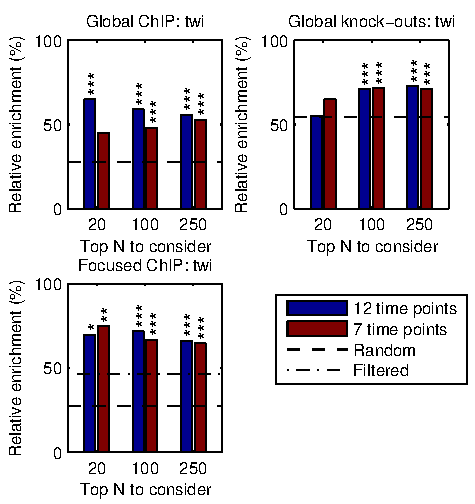
\includegraphics{dros_data_size_evaluation}
  \caption{Evaluation results similar to those in 
    Figs.~\ref{fig:dros_global_evaluation} and 
    \ref{fig:dros_focused_evaluation} for single-target models
    for full data (12 time points) and sub-sampled data (7 time points).
    \label{fig:dros_data_size_evaluation}
  }
\end{figure}

\section{Discussion}

We have shown how a very simple regulation model can be used to rank
genes according to their likelihood of being targeted by a specific
TF. The linear differential equation model of regulation we use is a simplification, and in
many cases unrealistic, but it can capture important differences in
the profiles of target genes due to differences in protein and mRNA
stability while still keeping the computational load at a level
that allows us to perform genome-wide scoring using a workstation
rather than a supercomputer. Our results show
that the model-based approach presented here can outperform the use of
loss-of-function mutant data for identifying targets. Such an approach
can be combined with binding location (ChIP-chip or ChIP-seq)
and spatial expression data to identify a confident set of regulatory
targets. This is especially useful in cases where loss-of-function
mutants are uninformative, either due to redundancy or because they do
not display a phenotype of interest. 

The main novelty of our approach is the use of recently proposed
techniques to model a time-varying degree of freedom as a sample from
a Gaussian process prior distribution~\cite{Gao2008}. By integrating out this functional
degree of freedom before computing the likelihood, we keep the
number of model parameters to a minimum and this allows us to model
typical short wild-type time series without excessive over-fitting. In
many applications it is difficult or impossible to achieve a high
degree of temporal resolution. For example, in studies of
embryogenesis it is often impossible to stage embryos with the
precision sufficient to obtain a long expression time series over the
period of interest. For one reason or another most expression time
series datasets are short~\cite{Ernst2005} and developing inference approaches
that are applicable to short time series datasets is of great
practical importance.  

Related methods have been proposed for identifying the
targets of a TF using time series expression data but few of these are suitable given the
limited data considered here~\cite{Bansal2007a}. Our approach was inspired by the work of Barenco {\em et
al.} who also use a differential equation with a linear activation
function to model the regulation of transcription. They focus on the
case where the TF is activated post-translation and they therefore
require the use of a training set of
known targets to infer the TF activity~\cite{Barenco2006a}. In the most recent
implementation of their method~\cite{Barenco2009} the original Markov
chain Monte Carlo procedure for Bayesian inference has been dropped due to its computational
inefficiency and an alternative optimisation-based method is used. In our case a Bayesian treatment of the TF protein
concentration is computationally efficient because we use Gaussian
process inference techniques. A Bayesian approach reduces the number of parameters
to be optimised, since we marginalise over the TF concentration, and
thereby reduces the possibility of over-fitting. Nevertheless, the use of a training set to infer the
TF concentration from targets was a very elegant solution to the
problem of dealing with TFs activated post-translation. This
approach also fits very naturally into the Gaussian process
framework as we have shown~\cite{Gao2008}. Such a scheme was unnecessary in the application considered
here, where the TFs of interest were known to be transcriptionally
regulated, but can be applied using our techniques in other
contexts. Unfortunately it is difficult for us to compare our method
directly with the results of Barenco {\em et al.} since their results
were only validated using the positive and negative targets that they identified,
rather than an unbiased test set. 

Another relevant method was introduced by Della Gatta {\em et
  al.}~\cite{Gatta2008}. They also use a linear regulation model but
they introduce simplifications that avoid the explicit solution of
differential equations. An interesting aspect of their approach is the
inclusion of a regulatory network model designed to capture the effect
of indirect regulation of putative targets by other genes. Sparse regression
techniques are used to learn the regulation model. A limitation of
their approach is the necessity to have measurements of the TF
protein; such data are not readily available in most cases. As with
Barenco's approach it is difficult for us to compare performance on
the data they used in~\cite{Gatta2008} because they only validated
selected predictions of their model. In our application we do not have
access to any protein data and therefore cannot apply their method as
intended. We were interested in whether
their approach to modelling indirect regulation would be helpful in
our case. Therefore we applied their approach using mRNA data as a
proxy for protein data which is not unreasonable for TFs under
transcriptional control. The results were no better than
using correlation with TF concentration. However, this comparison is
not fair to their method which really relies on the
availability of protein measurements.

There are some interesting differences in the ranking results for the two TFs studied
here. The knock-out scores for Twist are found to be less informative
about binding location than the knock-out scores for Mef2. This may be
because Twist acts earlier and therefore has many more indirect
downstream targets in the regulatory network. Indeed, Mef2 is a
direct target of Twist and therefore the direct targets of Mef2 are
indirect targets of Twist. These indirect targets will be
differentially expressed in the mutant and will therefore increase the
false positive rate. We also found that the model-based score results
for Mef2 show less improvement over the correlation score results in comparison to the Twist
results. Again, this can be explained by the fact that Mef2 is
later peaking. Targets activated by Mef2 are regulated towards the end of the
time period covered by the expression data used here. Therefore, there
are less data points available to capture the diversity of profiles
that can be explained by the regulation model. Conversely, the
correlation score is much less useful for Twist, since it misses many
targets that have profiles very different from the Twist mRNA
profile. 

We are pursuing a number of extensions of the current work. Here, we
have limited ourselves to detecting the targets of transcriptional activators. The
Gaussian process approach can be used to compute the likelihood for
repression models~\cite{Gao2008}. However, since models of repression
are inherently non-linear, the likelihood calculation is no longer analytically
tractable. Therefore approximate Bayesian inference methods are
required and we are currently working on an efficient implementation
for genome-wide ranking. We have also limited our attention
to single input motif models, but many targets will be regulated by other TFs and
co-factors. It seems doubtful that more complex models of regulation
will be useful for target ranking using only short wild-type time
series data, since it is unlikely these data would be sufficient to parametrise more complex models. However,
more general regulation models may be applicable if we were to use more data for
inferring the model parameters, e.g. time series knock-out data and time series
ChIP data could be highly informative. Scoring multiple input
models moves us closer to the more general gene regulatory network inference
problem. We expect that Gaussian processes will provide a useful way
to deal with inference over time-varying external inputs in these and other
biological systems.

\subsection{Availability}
Matlab code used in the experiments is available at
\texttt{http://www.cis.hut.fi/ahonkela/gpdisim/}.  An R implementation of
the ranking method is available from the authors upon request.

\begin{materials}
  \section{Expression data preprocessing} Drosophila developmental
  microarray time series from~\cite{Tomancak2002} were reprocessed
  using mmgMOS from the puma package~\cite{Pearson2009}.  The means of
  the log-scale expression values were equalized across chips.  The
  distributions over log-expression were transformed to means
  $\left(\hat{m}_i(t_j), \hat{f}_i(t_j)\right)$ and variances $\left(\sigma_{ijm}^2,
  \sigma_{if}^2 \right)$ of absolute expression by minimising the squared
  deviation of 5\%, 25\%, 50\%, 75\% and 95\% quantiles of a Gaussian
  distribution to corresponding quantiles obtained from mmgMOS.

  \section{Filtering quiet genes}
  Quiet genes can affect the ranking because any model with low or zero sensitivity can fit them
  well. Genes $j$ with an average z-score 
  $$ \frac{1}{Rn} \sum_{r=1}^R \sum_{i=1}^n \frac{\hat{m}_{jr}(t_i)}{\sigma_{ijr}} < 1.8 $$
  were considered quiet and removed from the data set.  The threshold
  was selected by visually inspecting models for candidate targets:
  practically all targets below the threshold elicited a
  non-informative constant response from the model.
  
  \section{Covariance of the Gaussian Process}
  Under suitable initial conditions, the differential
  equations~[\ref{eq:translation_ode}--\ref{eq:transcription_ode}]
  can be solved to obtain
  \begin{align*}
    %\label{eq:gpsim_f_ode_sol}
    p(t) &= \exp(-\delta t) \int_0^t f(v) \exp(\delta v) dv\ , \\
    m_j(t) &= \frac{B_j}{D_j} + S_j \exp(-D_j t) \int_0^t p(u)
    \exp(D_j u) du\ .
    %\label{eq:gpsim_f_x_sol}
  \end{align*}
  Using these solutions and assuming a squared exponential covariance
  for $f(t)$, $k_{ff}(t, t') = a \exp( -(t-t')^2/l^2)$, the covariance of target mRNAs is
  \begin{multline*}
    k_{m_j m_k}(t, t')
    = \frac{\sqrt{\pi} l a^2 S_j S_k}{2} \bigg(
    h_{jk}(t, t', \delta) + h_{kj}(t', t, \delta) \\
    - h_{jk}(t, t', D_j) - h_{kj}(t', t, D_k)
    \bigg)\ ,
  \end{multline*}
  where
  \begin{multline*}
    h_{jk}(t, t', D_x) = 
    \exp\left(\gamma_x^2\right)
    \frac{\exp(-D_x t - D_k t')}{(D_x + \delta) (D_j - \delta)}
    \bigg\{ 
    \\
    % \frac{(D_k + \delta)\exp((D_k-\delta) t') - 2\delta}{(D_k^2-\delta^2)}
    \left(\frac{\exp((D_k-\delta) t') - 1}{D_k-\delta} +
      \frac{1}{D_k + D_x} \right)
    \left[\erf\left(\gamma_x - \frac{t}{l}\right) - \erf\left(\gamma_x\right)\right]
    \\
    + \frac{\exp((D_k+D_x)t')}{D_k+D_x}
    \left[\erf\left(\gamma_x + \frac{t'}{l}\right)
    - \erf\left(\gamma_x - \frac{\Delta t}{l}\right)\right]
    \bigg\}\ ,
  \end{multline*}
  where $\Delta t := t - t'$ and $\gamma_x = \frac{D_x l}{2}$.
  Similarly, 
  \begin{multline*}
    k_{f m_k}(t, t')
    = \frac{\sqrt{\pi} l a^2 S_k}{2(\delta - D_k)} \\
    \bigg\{
    \exp\left(\gamma_k^2 + D_k \Delta t \right)
    \left[\erf\left(\gamma_k + \frac{t}{l}\right) - \erf\left(\gamma_k + \frac{\Delta t}{l}\right)\right] \\
    -
    \exp\left(\gamma_\delta^2 + \delta \Delta t\right)
    \left[\erf\left(\gamma_\delta + \frac{t}{l}\right) - \erf\left(\gamma_\delta + \frac{\Delta t}{l}\right)\right]
    \bigg\}\ ,
  \end{multline*}
  where $\gamma_k = \frac{D_k l}{2}$ and $\gamma_\delta = \frac{\delta l}{2}$.

  \section{Training set ranking}
  The training set or multiple-target ranking was formed by fitting
  joint models to five assumed known targets together with each new
  candidate independently and ranking by model likelihood.  In our
  approach, the training set was formed by taking 5 highest-ranking
  targets from the single-target method, but naturally any existing background
  knowledge of known targets should be utilised.  To speed up the
  computation, we first fitted a Gaussian process model to the
  training set genes alone.  All the parameters concerning these genes
  were then fixed when fitting the larger models to the training set
  plus each candidate.

  \section{Knock-out data processing}
  The knock-out data was processed as explained
  in~\cite{Sandmann2006a}.  $q$-values were computed at each time
  point using SAM~\cite{Saeed2003,Tusher2001}, the values at
  neighbouring time points were averaged and the minimum of these
  averages was used as the final value.  A cut-off value of 0.1 was
  used for detecting significant differential expression as
  in~\cite{Sandmann2006a}.

\end{materials}

\begin{acknowledgments}
A.H. was supported by Postdoctoral Researcher's Project No 121179 of the Academy of Finland.
M.R. and N.D.L acknowledge support from EPSRC Grant No EP/F005687/1 "Gaussian Processes for Systems Identification with Applications in Systems Biology". 
This work was supported in part by the IST Programme of the European Community, under the PASCAL2 Network of Excellence, IST-2007-216886. This publication only reflects the authors' views.
\end{acknowledgments}

\bibliographystyle{pnas}
\bibliography{disim}

%\begin{thebibliography}{10}
%\bibliography{puma_package}
%\end{thebibliography}
\end{article}

% Figures


\end{document}


